\documentclass[11pt]{article}
    \usepackage{caption}
    \usepackage{graphicx}
    \usepackage{mathtools}
    \setlength{\parindent}{0pt}
    \DeclareCaptionType{equ}[][]
    \usepackage[svgnames]{xcolor}
    
    \newcommand*{\plogo}{\fbox{$\mathcal{BM}$}}
    
    \usepackage{PTSerif}
    
    \begin{document} 
        
    \begin{titlepage}
    
        \raggedleft
        
        \vspace*{\baselineskip}
        
        {\Large Bryan Melanson}
        
        \vspace*{0.167\textheight}
        
        \textbf{\LARGE How to Not Fail}\\[\baselineskip]
        
        {\textcolor{Red}{\Huge Control Systems}}\\[\baselineskip]
        
        {\Large \textit{While never going to class}}
        
        \vfill
        
        {\large Computer Engineering 2020 ~~\plogo}
        
        \vspace*{3\baselineskip}
    
    \end{titlepage}

    \pagebreak
    
    \tableofcontents

    \section{Modelling}
    \section{Time Response}
    \section{Systems Reduction}
    \section{Stability}
    \subsection{Routh Hurwitz}
    \begin{center}
        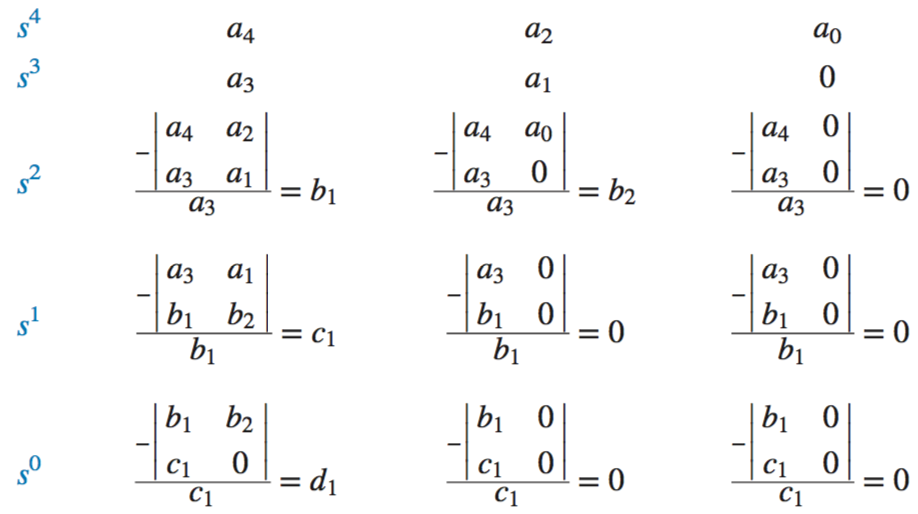
\includegraphics[width = 300 px]{img/routh}        
    \end{center}
    \subsubsection{Zero Only in First Column}
    \begin{center}
        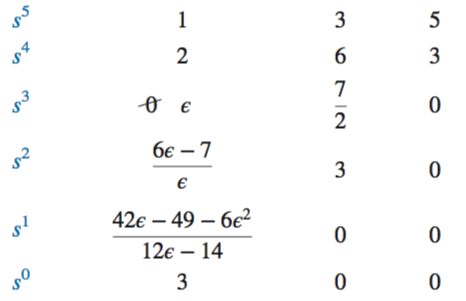
\includegraphics[width = 300 px]{img/routh-e}        
    \end{center}
    \begin{center}
        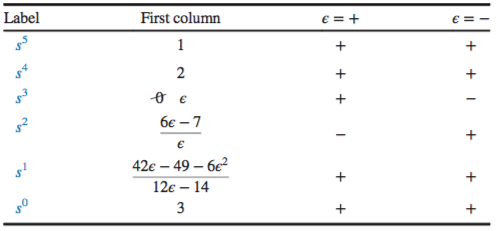
\includegraphics[width = 300 px]{img/routh-e2}        
    \end{center}
    \subsubsection{Entire Row of Zeroes}
    \subsubsection{Reverse Coefficients}
    \begin{center}
        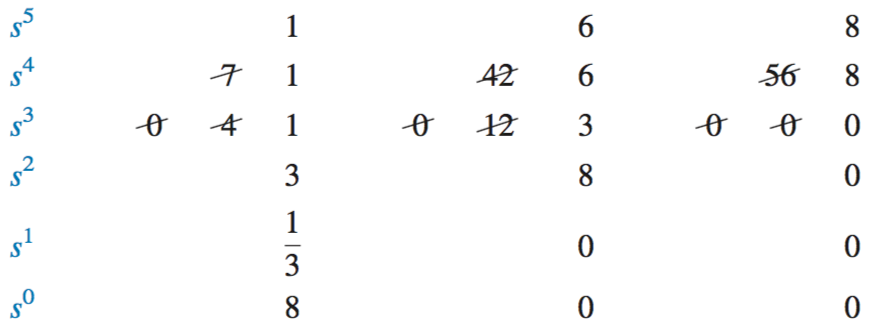
\includegraphics[width = 300 px]{img/routh-roz}        
    \end{center}
    \subsection{Stability in State Space}
    \section{Steady State}
    \section{Root Locus}
    \section{Root Locus Design}
    \section{Frequency Response}
    \section{Digital Control}

    \end{document}